\documentclass[11pt]{article}
\usepackage[a4paper,margin=2.5cm]{geometry}
\usepackage{amsmath,amsfonts,amssymb}
\usepackage{graphicx}
\usepackage{hyperref}
\usepackage{listings}
\usepackage{color}
\usepackage{caption}
\usepackage{float}
\usepackage{booktabs}
\usepackage{fancyhdr}
\usepackage{enumitem}
\usepackage[official]{eurosym}

\AddToHook{cmd/section/before}{\clearpage}

\pagestyle{fancy}
\fancyhf{}
\rhead{Flexibility Study Guide}
\lhead{RSE Research Preparation}
\rfoot{\thepage}

%\hypersetup{
%	colorlinks=true,
%	linkcolor=blue,
%	citecolor=blue,
%	urlcolor=blue
%}

\title{Technical Study Guide\\for Local Flexibility Services in Distribution Networks}
\author{Prepared by: Marco Donà}
\date{\today}

\begin{document}
	
	\maketitle
	\tableofcontents
	\newpage
	
	% ===================================================================
	\section{Introduction}
	
	\subsection*{Objectives of the Study}
	
	The objective of this document is to serve as a comprehensive technical guide for the preparation of a research-oriented interview at \textbf{RSE – Ricerca sul Sistema Energetico}, focusing on the position \textit{“Simulation and experimentation of schemes for local flexibility services” (Ref. TGM7\_2025\_RAC)}.
	
	The document consolidates theoretical foundations, computational methods, and practical insights spanning distribution network modeling, power flow analysis, flexibility mechanisms, and control theory.  
	It is designed to enable a deep and structured understanding of the multidisciplinary topics relevant to this research area, bridging electrical engineering, optimization, and automation.
	
	The final goal is to achieve:
	\begin{itemize}
		\item A solid grasp of the physical and mathematical models underlying distribution networks.
		\item The ability to simulate and analyze power flow and flexibility activation using numerical tools.
		\item Understanding of the regulatory and market context for local flexibility in Europe and Italy.
		\item The capability to apply control and optimization methods to power system operation problems.
	\end{itemize}
	
	\subsection*{Position Requirements Overview}
	
	According to RSE’s call for applications (Ref. TGM7\_2025\_RAC, 2025), the role requires a multidisciplinary background including:
	\begin{itemize}
		\item Modeling and simulation of electrical distribution networks, including \textit{Power Flow} and \textit{Optimal Power Flow (OPF)} analysis.
		\item Understanding of electricity markets and regulatory frameworks, particularly concerning DSOs and ancillary services.
		\item Knowledge of optimization and control techniques for energy systems.
		\item Familiarity with scientific programming environments (MATLAB, Python, Julia).
	\end{itemize}
	
	Preferred qualifications also include experience in:
	\begin{itemize}
		\item Research projects funded by national or European programs (e.g., Horizon, PNRR).
		\item Advanced control (predictive, optimal, robust) and optimization techniques.
		\item Simulation tools such as DIgSILENT PowerFactory, OpenDSS, or MATPOWER.
	\end{itemize}
	
	The skills covered in this document align with these requirements, providing both theoretical explanations and practical examples to support technical discussion during the interview.
	
	\subsection*{How This Document Is Structured}
	
	The document follows a progressive learning structure, starting from fundamental principles and advancing toward complex interdisciplinary applications:
	
	\begin{enumerate}
		\item \textbf{Fundamentals of Distribution Networks} – topology, components, and per-unit modeling.
		\item \textbf{Power Flow and Optimal Power Flow} – steady-state analysis and optimization.
		\item \textbf{Flexibility in Distribution Networks} – modeling, classification, and quantification.
		\item \textbf{Electricity Markets and Regulation} – European and Italian frameworks for local flexibility.
		\item \textbf{Optimization Techniques} – from convex to mixed-integer and stochastic methods.
		\item \textbf{Control Theory and Automation} – predictive and hierarchical control for smart grids.
		\item \textbf{Simulation Tools and Programming} – Python, MATLAB, and power system simulators.
		\item \textbf{Research Methodology and Project Participation} – good practices in scientific collaboration.
	\end{enumerate}
	
	Each section concludes with key concepts, equations, and references to primary sources such as:
	\begin{itemize}
		\item IEEE standards and textbooks on power systems and control.
		\item ENTSO-E and ARERA regulatory documents.
		\item RSE and EU project reports on local flexibility and grid automation.
	\end{itemize}
	
	This document aims to be self-contained yet rigorous, serving as both a study manual and a future technical reference for applied research in electrical energy systems.
	
	
	% ===================================================================
	\section{Fundamentals of Distribution Networks}
	
	\subsection{Structure and Components}
	
	A power distribution network is the final stage in the electrical power system, delivering electricity from transmission substations to end-users.  
	Its structure reflects the transition from high-voltage (HV) transmission systems to medium-voltage (MV) and low-voltage (LV) grids.
	
	\begin{itemize}
		\item \textbf{Transmission network}: typically operates above 110~kV, designed for long-distance bulk power transfer.
		\item \textbf{Primary distribution (MV)}: ranges from 1~kV to 35~kV, connecting substations to local feeders.
		\item \textbf{Secondary distribution (LV)}: below 1~kV, supplying residential, commercial, and industrial loads.
	\end{itemize}
	
	The main components of a distribution network are:
	\begin{itemize}
		\item \textbf{Transformers} – step-down voltage levels between stages (HV/MV/LV).
		\item \textbf{Feeders and laterals} – overhead or underground conductors that deliver power to customers.
		\item \textbf{Switches, circuit breakers, and protection devices} – ensure safe operation and fault isolation.
		\item \textbf{Distributed Energy Resources (DERs)} – local generators (e.g., PV, wind), storage, and demand-side resources.
		\item \textbf{Smart meters and sensors} – provide data for monitoring, automation, and flexibility services.
	\end{itemize}
	
	Modern distribution systems are evolving toward \textbf{active distribution networks (ADNs)}, in which distributed resources and controllable loads participate in voltage regulation, congestion management, and flexibility provision \cite{ENTSOE_flexibility2023,CIRED_ADN2019}.
	
	\subsection{Radial vs. Meshed Networks}
	
	Traditionally, distribution networks have been designed as \textbf{radial systems}, where power flows unidirectionally from the substation to the end users.  
	In a radial feeder, each load is supplied by a single path, which simplifies protection coordination and reduces system cost.
	
	However, the increasing penetration of distributed generation (DG) and storage has motivated the development of \textbf{meshed or looped topologies}, providing multiple paths for power flow and improved reliability.  
	These configurations, though more complex to control, enable bidirectional power exchange and facilitate flexibility activation.
	
	The network topology can be characterized by its \textit{graph representation}:
	\[
	\mathcal{G} = (\mathcal{N}, \mathcal{E})
	\]
	where $\mathcal{N}$ is the set of buses (nodes) and $\mathcal{E}$ is the set of lines (edges).  
	For radial networks, $|\mathcal{E}| = |\mathcal{N}| - 1$, while meshed systems contain additional loops, i.e. $|\mathcal{E}| > |\mathcal{N}| - 1$.
	
	\subsection{Per Unit System and Base Values}
	
	To simplify power system analysis, electrical quantities are often expressed in the \textbf{per unit (p.u.) system}.  
	This normalization makes equations dimensionless and allows easy comparison across different voltage levels.
	
	For a given system base:
	\[
	S_\text{base} = \text{apparent power base (MVA)}, \quad V_\text{base} = \text{voltage base (kV)}
	\]
	the derived quantities are:
	\[
	I_\text{base} = \frac{S_\text{base}}{\sqrt{3}V_\text{base}}, \quad Z_\text{base} = \frac{V_\text{base}^2}{S_\text{base}}
	\]
	Then any quantity $X$ (voltage, current, impedance, power) can be expressed as:
	\[
	X_{pu} = \frac{X_\text{actual}}{X_\text{base}}
	\]
	This approach simplifies multi-voltage network calculations, especially when transformers are involved, since all elements can be converted to a common base \cite{kundur1994power,grainger1994power}.
	
	\subsection{Load Models and Profiles}
	
	Load modeling is a key aspect of distribution network studies.  
	Different load models capture how demand responds to voltage and frequency variations, influencing voltage stability and flexibility assessments.
	
	\subsubsection*{Static load models}
	Static models relate active and reactive power to voltage magnitude:
	\[
	P = P_0 \left( \frac{V}{V_0} \right)^{\alpha}, \quad Q = Q_0 \left( \frac{V}{V_0} \right)^{\beta}
	\]
	where $\alpha$ and $\beta$ define the voltage dependence:
	\begin{itemize}
		\item Constant power load: $\alpha = \beta = 0$
		\item Constant current load: $\alpha = \beta = 1$
		\item Constant impedance load: $\alpha = \beta = 2$
	\end{itemize}
	
	\subsubsection*{Dynamic load models}
	Dynamic models consider time-dependent behavior, including thermostatically controlled loads, electric vehicles (EVs), and heat pumps.  
	These loads introduce temporal flexibility, allowing demand shifting or curtailment during grid operation.
	
	\subsubsection*{Load profiles}
	Typical LV or MV load profiles vary by consumer type:
	\begin{itemize}
		\item \textbf{Residential:} peak in the evening (18–22 h).
		\item \textbf{Commercial:} peak during daytime hours.
		\item \textbf{Industrial:} relatively constant demand.
	\end{itemize}
	Profiles are often normalized and derived from measurement campaigns or standard datasets (e.g., ENTSO-E, TERNA, EDSO).  
	In flexibility studies, load profiles are crucial for estimating baseline consumption and available flexibility.
	
	\subsection*{Summary}
	
	This section has introduced the structure, modeling, and representation of distribution networks, providing the foundation for subsequent analysis such as Power Flow and Optimal Power Flow (OPF).  
	The next section will build on these concepts, describing the mathematical formulation of power flow equations and optimization-based extensions.
	
	
	% ===================================================================
	\section{Power Flow and Optimal Power Flow}
	
	\subsection{AC and DC Power Flow}
	
	The \textbf{Power Flow Problem} (also known as \textit{Load Flow}) is a fundamental tool in power system analysis.  
	It determines the steady-state operating condition of a network, i.e. bus voltages, line currents, and power flows, given a specified load and generation scenario.
	
	A power system can be represented as a network of buses connected by transmission or distribution lines.  
	At each bus $i$, the complex power injection is given by:
	\[
	S_i = P_i + jQ_i = V_i I_i^*
	\]
	where $V_i=|V_i|e^{j\delta_i}$ is the complex bus voltage and $I_i^*$ is the conjugate of the injected current.
	
	By applying Kirchhoff’s Current Law (KCL) and using the network admittance matrix $Y_{bus}$, the relationship becomes:
	\[
	I_i = \sum_{j=1}^N Y_{ij} V_j
	\]
	Substituting, we obtain the nonlinear power flow equations:
	\[
	S_i = V_i \sum_{j=1}^N Y_{ij}^* V_j^*
	\]
	or, separating into active and reactive power components:
	\[
	\begin{aligned}
		P_i &= \sum_{j=1}^N |V_i||V_j| \left( G_{ij} \cos\theta_{ij} + B_{ij} \sin\theta_{ij} \right) \\
		Q_i &= \sum_{j=1}^N |V_i||V_j| \left( G_{ij} \sin\theta_{ij} - B_{ij} \cos\theta_{ij} \right)
	\end{aligned}
	\]
	where:
	\begin{itemize}
		\item $G_{ij}$ and $B_{ij}$ are the conductance and susceptance between buses $i$ and $j$,
		\item $\theta_{ij} = \delta_i - \delta_j$ is the phase angle difference.
	\end{itemize}
	
	Solving these nonlinear equations provides:
	\begin{itemize}
		\item Bus voltage magnitudes and angles;
		\item Real and reactive power flows on each line;
		\item System losses.
	\end{itemize}
	
	\subsubsection*{Bus types}
	
	To solve the power flow problem, bus types must be defined:
	\begin{itemize}
		\item \textbf{Slack (reference) bus:} $V$ and $\delta$ known; $P$, $Q$ computed.
		\item \textbf{PV bus:} $P$ and $|V|$ known; $\delta$, $Q$ computed.
		\item \textbf{PQ bus:} $P$, $Q$ known; $|V|$, $\delta$ computed.
	\end{itemize}
	
	\subsubsection*{Numerical solution methods}
	
	The most common iterative techniques are:
	\begin{itemize}
		\item \textbf{Gauss-Seidel} — simple but slow convergence.
		\item \textbf{Newton-Raphson (NR)} — quadratic convergence; standard for large systems.
		\item \textbf{Fast-Decoupled Load Flow (FDLF)} — approximated NR using decoupled $P$–$\theta$ and $Q$–$V$ subproblems.
	\end{itemize}
	
	In MATLAB or Python environments, these are implemented in tools such as \texttt{MATPOWER} \cite{zimmerman2011matpower} and \texttt{pandapower}.
	
	\subsubsection*{DC Power Flow Approximation}
	
	The DC power flow is a linearized approximation valid under:
	\begin{enumerate}
		\item Small angle differences ($\sin\theta \approx \theta$).
		\item Voltage magnitudes near 1 p.u. ($|V| = 1$).
		\item Negligible line resistance ($R \ll X$).
	\end{enumerate}
	
	Under these assumptions:
	\[
	P_i = \sum_{j} B_{ij} (\delta_i - \delta_j)
	\]
	This simplification allows very fast computation, suitable for market clearing, contingency screening, and optimization problems such as OPF or flexibility dispatch.
	
	\subsection{Optimal Power Flow (OPF): Introduction}
	
	The \textbf{Optimal Power Flow} (OPF) problem extends the traditional power flow by optimizing a given objective function (e.g., minimizing cost or losses), while satisfying physical and operational constraints.
	
	The generic OPF formulation is:
	\[
	\begin{aligned}
		\min_{x,u} \quad & f(x,u) \\
		\text{s.t.} \quad & g(x,u) = 0 \quad \text{(power flow equations)}\\
		& h(x,u) \le 0 \quad \text{(operational constraints)}
	\end{aligned}
	\]
	where:
	\begin{itemize}
		\item $x$ = state variables (voltages, angles),
		\item $u$ = control variables (generator outputs, tap changers, flexible loads),
		\item $f(x,u)$ = objective function (e.g., generation cost, losses, voltage deviation).
	\end{itemize}
	
	\textbf{Common objectives:}
	\begin{itemize}
		\item $\min \sum_i C_i(P_{G_i})$ — generation cost minimization;
		\item $\min \sum_{(i,j)} r_{ij} I_{ij}^2$ — loss minimization;
		\item $\min \sum_i |V_i - V_{ref}|^2$ — voltage regulation;
		\item $\max$ renewable utilization or flexibility activation.
	\end{itemize}
	
	\textbf{Typical constraints:}
	\begin{align*}
		P_i^{G} - P_i^{D} &= \sum_{j} |V_i||V_j|(G_{ij}\cos\theta_{ij} + B_{ij}\sin\theta_{ij}) \\
		Q_i^{G} - Q_i^{D} &= \sum_{j} |V_i||V_j|(G_{ij}\sin\theta_{ij} - B_{ij}\cos\theta_{ij}) \\
		V_i^{\min} &\le |V_i| \le V_i^{\max} \\
		P_i^{G,\min} &\le P_i^{G} \le P_i^{G,\max} \\
		S_{ij} &\le S_{ij}^{\max}
	\end{align*}
	
	\subsubsection{Interpretation of the Constraints}
	
	\paragraph{1. Active power balance.}
	\[
	P_i^{G} - P_i^{D} = \sum_{j} |V_i||V_j|(G_{ij}\cos\theta_{ij} + B_{ij}\sin\theta_{ij})
	\]
	This equation ensures that the \textbf{net active power} injected at bus $i$ (generation minus demand) equals the sum of all active power flows from bus $i$ to its connected neighbors. It enforces the conservation of real power in the steady state.
	
	\paragraph{2. Reactive power balance.}
	\[
	Q_i^{G} - Q_i^{D} = \sum_{j} |V_i||V_j|(G_{ij}\sin\theta_{ij} - B_{ij}\cos\theta_{ij})
	\]
	This represents the equilibrium of reactive power at each bus. Reactive power affects the voltage profile of the system, and this constraint ensures proper voltage support and system stability.
	
	\paragraph{3. Voltage magnitude limits.}
	\[
	V_i^{\min} \le |V_i| \le V_i^{\max}
	\]
	Each bus voltage must stay within permissible limits (typically between 0.95 and 1.05 p.u.). This constraint guarantees quality of supply and avoids voltage instability or damage to equipment.
	
	\paragraph{4. Generator limits.}
	\[
	P_i^{G,\min} \le P_i^{G} \le P_i^{G,\max}
	\]
	Every generator can operate only within its technical range. This constraint represents the physical capacity of each generating unit.
	
	\paragraph{5. Line flow limits.}
	\[
	S_{ij} \le S_{ij}^{\max}
	\]
	The apparent power flow on each line cannot exceed its thermal or stability limit. This ensures that no transmission element is overloaded, preserving safety and reliability.
	
	\subsection{Solving OPF: Convex Relaxations and Algorithms}
	
	The AC-OPF is a \textbf{nonconvex, nonlinear} optimization problem (due to quadratic equality constraints).  
	Several relaxation and approximation methods exist to improve computational tractability:
	
	\begin{itemize}
		\item \textbf{DC-OPF:} linearization assuming flat voltage magnitude and small angle differences.
		\item \textbf{Quadratic Programming (QP)} or \textbf{Linear Programming (LP)} for convex cost functions.
		\item \textbf{Second-Order Cone Programming (SOCP)} relaxation — convex approximation preserving voltage and current limits.
		\item \textbf{Semidefinite Programming (SDP)} relaxation — globally optimal under certain network conditions \cite{lavaei2012zero}.
	\end{itemize}
	
	Common solvers include:
	\begin{itemize}
		\item \texttt{IPOPT}, \texttt{CPLEX}, \texttt{GUROBI}, \texttt{MOSEK} (general-purpose);
		\item \texttt{MATPOWER}, \texttt{PYPOWER}, \texttt{pandapower}, and \texttt{Julia/JuMP} for OPF modeling.
	\end{itemize}
	
	\subsection{Applications in Flexibility Analysis}
	
	In the context of distribution networks, OPF can be extended to model the participation of flexible resources, such as demand response or distributed storage, in local markets.
	
	\textbf{Examples of flexibility-oriented objectives:}
	\begin{itemize}
		\item Minimizing voltage violations via demand curtailment;
		\item Minimizing DSO operational cost subject to network limits;
		\item Maximizing offered flexibility from DERs to resolve contingencies.
	\end{itemize}
	
	The optimization can include binary variables representing activation decisions (mixed-integer OPF), or stochastic components to account for renewable uncertainty.
	
	Mathematically, flexibility activation can be formulated as:
	\[
	\min_{P_{G}, P_{flex}} \quad C(P_{G}) + C_{flex}(P_{flex})
	\]
	subject to power balance and operational constraints, where $P_{flex}$ represents controllable flexibility provision (positive or negative power modulation).
	
	\subsection{Tools: MATPOWER, OpenDSS, PowerFactory (Overview)}
	
	\textbf{MATPOWER} \cite{zimmerman2011matpower} is an open-source MATLAB toolbox for steady-state power flow and OPF analysis.  
	It supports both AC and DC formulations and is widely used in academia.
	
	\textbf{OpenDSS} (Open Distribution System Simulator) is developed by EPRI for distribution-level studies.  
	It includes time-series simulations, integration with Python, and support for smart grid applications such as voltage control and storage management.
	
	\textbf{DIgSILENT PowerFactory} is a commercial-grade simulator offering advanced capabilities (dynamic studies, protection, market modeling).  
	It is often used in research projects and by DSOs for system planning and flexibility analysis.
	
	\subsection*{Summary}
	
	Power flow and OPF methods form the analytical foundation for evaluating flexibility in modern distribution systems.  
	While AC power flow provides the physical representation of network behavior, OPF integrates economic and operational optimization — essential for designing and analyzing local flexibility markets.
	
	
	% ===================================================================
	\section{Flexibility in Distribution Networks}
	
	\subsection{Definition and Importance}
	
	Flexibility in power systems refers to the ability of the electricity network and connected resources to adapt generation or consumption patterns in response to internal or external signals, such as market prices, grid constraints, or renewable generation variability.
	
	Formally, flexibility can be defined as:
	\[
	F(t) = \frac{dP(t)}{dt}
	\]
	representing the rate at which the net power exchange at a node (or network area) can be modified within technical and operational limits.
	
	Flexibility enables several key objectives:
	\begin{itemize}
		\item Maintaining balance between generation and demand in real time;
		\item Mitigating voltage or thermal limit violations in distribution grids;
		\item Integrating variable renewable generation (solar, wind);
		\item Supporting congestion management and system restoration;
		\item Providing local ancillary services to the DSO.
	\end{itemize}
	
	In the context of active distribution networks (ADNs), the DSO becomes an active system operator, coordinating local flexibility from distributed energy resources (DERs) to enhance system efficiency and reliability \cite{CEDEC2019_flexibility,entsoe2023_flexibility}.
	
	\subsection{Types of Flexible Resources}
	
	Flexibility can originate from different technologies and actors.  
	The main classes are listed below.
	
	\subsubsection*{Energy Storage Systems (ESS)}
	Storage systems such as batteries or thermal reservoirs can shift energy temporally, providing both upward (discharging) and downward (charging) flexibility.  
	Their main constraints are energy capacity ($E_\text{max}$), power limits ($P_\text{max}$), and state of charge (SOC):
	\[
	SOC(t+1) = SOC(t) + \eta_c P_\text{ch}(t)\Delta t - \frac{1}{\eta_d} P_\text{dis}(t)\Delta t
	\]
	with $0 \le SOC(t) \le E_\text{max}$.
	
	\subsubsection*{Demand Response (DR)}
	Demand-side flexibility comes from modulating consumption according to price signals or direct control commands.  
	DR can be:
	\begin{itemize}
		\item \textbf{Implicit (price-based):} customers react voluntarily to dynamic tariffs;
		\item \textbf{Explicit (contract-based):} aggregators or DSOs activate loads in exchange for payments.
	\end{itemize}
	Examples include HVAC systems, electric vehicles, or industrial processes with schedulable loads.
	
	\subsubsection*{Renewable Generation (Variable RES)}
	Photovoltaic (PV) and wind plants can provide downward flexibility by curtailing production.  
	Some inverter-based units also offer upward flexibility via reactive power control or temporary overproduction within rated limits.
	
	\subsubsection*{Virtual Power Plants (VPPs)}
	A \textbf{Virtual Power Plant} aggregates multiple DERs (generation, storage, flexible loads) and operates them as a coordinated entity.  
	The VPP can participate in markets and provide local services to the DSO while ensuring that network constraints are not violated \cite{mohandes2021vpp}.
	
	\subsubsection*{Energy Communities and Local Aggregators}
	\textbf{Renewable Energy Communities (RECs)} and \textbf{Citizen Energy Communities (CECs)} represent collective actors who manage distributed flexibility across prosumers.  
	Their aggregated potential can be used for peak shaving, congestion management, and energy self-sufficiency at the local level.
	
	\subsection{Activation Mechanisms and Signals}
	
	The activation of flexibility can occur through various control and market-based mechanisms.
	
	\begin{itemize}
		\item \textbf{Direct control:} the DSO or aggregator sends activation commands (e.g., load reduction of 50~kW for 15~minutes).
		\item \textbf{Price signals:} variable energy prices incentivize consumers to adjust demand autonomously.
		\item \textbf{Market-based dispatch:} flexibility bids/offers are submitted to a local market platform and cleared through an optimization (e.g., OPF or auction).
		\item \textbf{Emergency activation:} used in contingency situations, where system operators request immediate support.
	\end{itemize}
	
	The response can be characterized by:
	\begin{itemize}
		\item \textbf{Activation time ($t_\text{act}$):} delay between request and actual power change;
		\item \textbf{Duration ($T_\text{flex}$):} period for which the flexibility can be sustained;
		\item \textbf{Recovery time ($t_\text{rec}$):} period before the resource returns to its baseline state.
	\end{itemize}
	
	These parameters are crucial for defining flexibility products and evaluating the reliability of flexible resources.
	
	\subsection{Flexibility Potential Estimation}
	
	Estimating the \textit{potential} of flexibility in a distribution network involves assessing how much power variation ($\Delta P$, $\Delta Q$) can be achieved at each node or feeder, considering technical and network limits.
	
	Mathematically, the flexibility envelope at bus $i$ can be formulated as:
	\[
	\mathcal{F}_i = \left\{ (\Delta P_i, \Delta Q_i) \;|\; V_i^{\min} \le V_i \le V_i^{\max}, \; S_{ij} \le S_{ij}^{\max} \right\}
	\]
	In other words, $\mathcal{F}_i$ is a feasible region in the $P$-$Q$ plane containing all possible active and reactive power changes $(\Delta P_i,\Delta Q_i)$ that a node (bus)
	$i$ in the distribution network can provide without violating technical constraints.
	
	The total system flexibility is defined as:
	\[
	F_\text{sys}(t) = \sum_{i} \Delta P_i(t)
	\]
	subject to network constraints derived from an OPF model.
	
	\textbf{Approaches for estimation:}
	\begin{itemize}
		\item \textbf{Analytical methods:} linearized power flow sensitivities (Jacobian-based).
		\item \textbf{Optimization-based:} solving multiple OPF instances to derive upper/lower flexibility bounds.
		\item \textbf{Data-driven approaches:} regression or machine learning models trained on simulation data or historical measurements.
	\end{itemize}
	
	These methods can quantify not only the total available flexibility but also its \textbf{spatial} and \textbf{temporal} distribution, which are essential for DSO decision-making and local market design.
	
	\subsection{Multi-Energy Systems and Sector Coupling}
	
	Future flexibility solutions will increasingly rely on \textbf{multi-energy systems}, where electricity, heat, and gas sectors interact to provide cross-sector flexibility.
	
	Examples include:
	\begin{itemize}
		\item Using \textbf{heat pumps} and \textbf{thermal storage} to shift electrical demand through heat buffering.
		\item Employing \textbf{Power-to-Gas (P2G)} and \textbf{Power-to-Heat (P2H)} technologies to absorb surplus renewable energy.
		\item Integrating \textbf{electric vehicles (EVs)} as mobile storage units.
	\end{itemize}
	
	This concept is referred to as \textbf{sector coupling}, enabling additional degrees of flexibility across the energy system and supporting decarbonization goals \cite{IEA_sectorcoupling2021}.
	
	\subsection*{Summary}
	
	Flexibility in distribution networks is a cornerstone of the energy transition.  
	It bridges technical control and economic optimization, enabling distributed energy resources and consumers to actively participate in system operation.  
	Understanding how to model, quantify, and activate flexibility — both from the network and market perspectives — is central to research roles such as the one at RSE.
	
	
	% ===================================================================
	\section{Electricity Markets and Regulation}
	
	\subsection{Introduction}
	
	Electricity markets provide the economic framework within which generation, consumption, and flexibility interact.  
	They ensure that energy is produced, transported, and consumed efficiently while maintaining system reliability and promoting competition.  
	In Europe, the market structure has evolved to integrate renewable sources and decentralized actors, leading to the emergence of new products such as local flexibility and ancillary services.
	
	This section introduces the fundamental market architecture, key regulatory principles, and the evolving role of Distribution System Operators (DSOs) and aggregators.
	
	\subsection{Market Structure Overview}
	
	The European power market is organized into multiple temporal and spatial layers, as illustrated in Figure~\ref{fig:market_layers}.  
	Each layer corresponds to a specific time horizon and operational objective.
	
	\begin{figure}[ht]
		\centering
		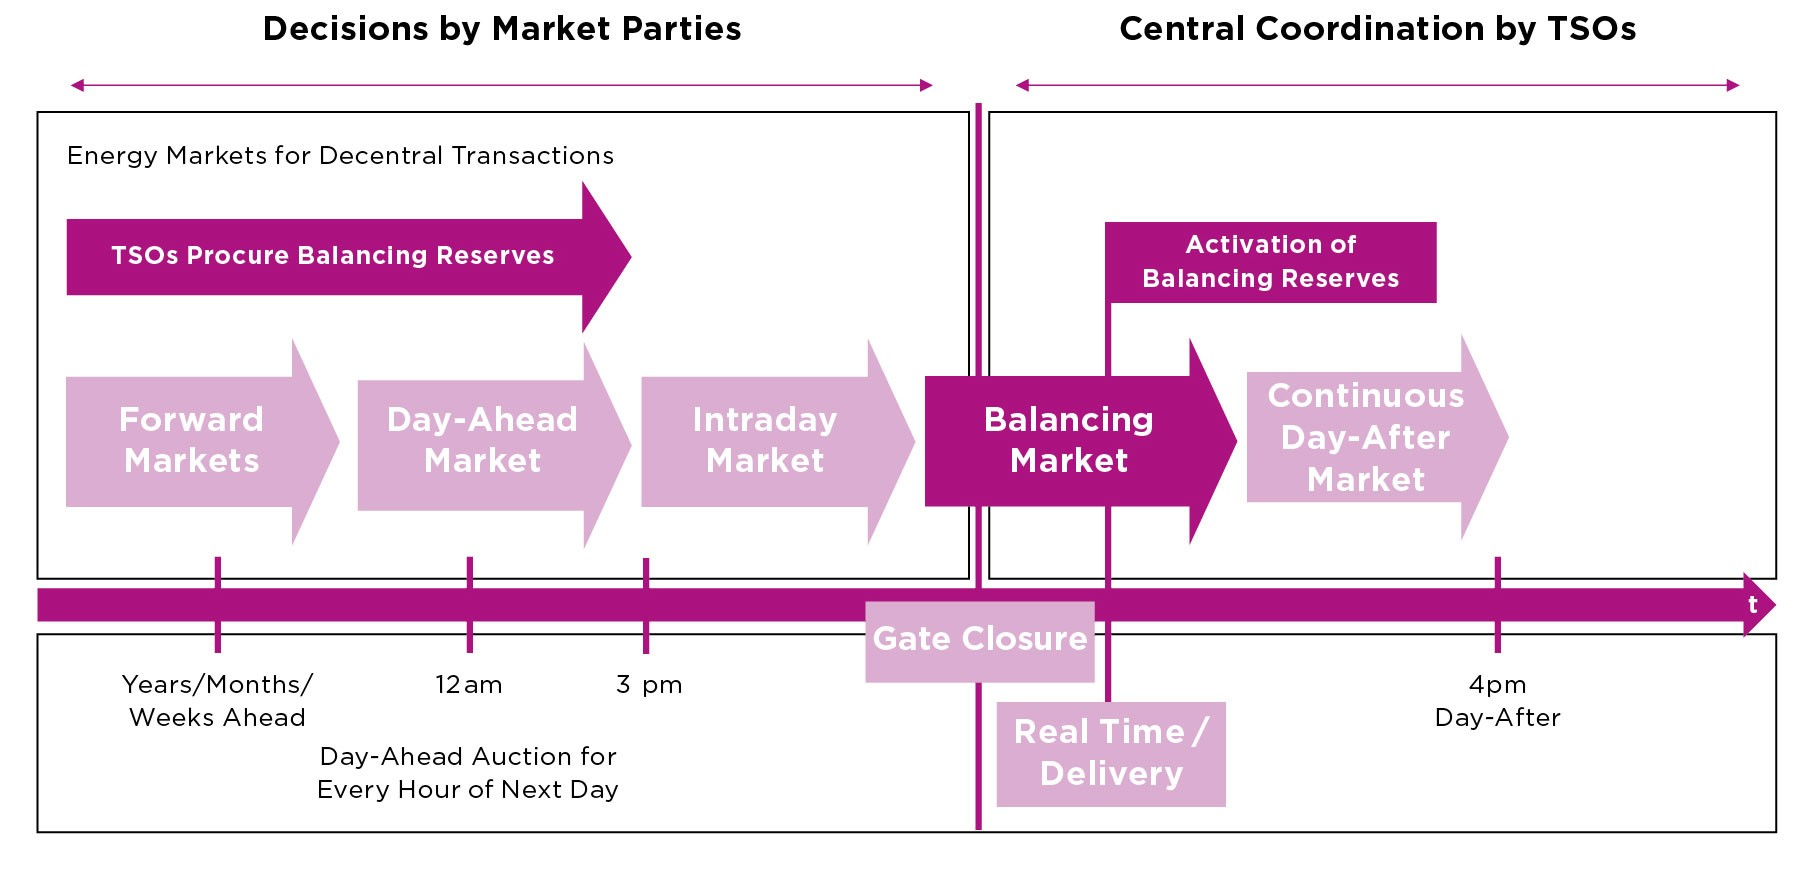
\includegraphics[width=0.7\linewidth]{images/european_electricity_market_layers}
		\caption{Overview of different timeframes of the wholesale and balancing markets.}
		\label{fig:market_layers}
	\end{figure}
	
	
	\begin{itemize}
		\item \textbf{Forward / Futures Market:} contracts for months or years ahead; used for hedging price risks.
		\item \textbf{Day-Ahead Market (DAM):} determines the energy schedule for each hour of the next day through a market coupling algorithm (EUPHEMIA).
		\item \textbf{Intraday Market (IDM):} enables trading closer to real time to adjust for forecast errors.
		\item \textbf{Balancing Market (BM):} operated by the Transmission System Operator (TSO) to correct imbalances in real time.
		\item \textbf{Local Flexibility Markets (LFM):} emerging platforms where DSOs procure flexibility to solve local constraints.
	\end{itemize}
	
	\begin{equation}
		\text{Time Horizon:} \quad \text{Years} \rightarrow \text{Day-Ahead} \rightarrow \text{Intraday} \rightarrow \text{Real-Time}
	\end{equation}
	
	\subsection{Day-Ahead Market (DAM)}
	
	The \textit{Day-Ahead Market} (DAM) is a \textbf{centralized auction} in which electricity market participants submit energy bids and offers for each hour of the following day.  
	In Italy, this market is managed by the \textbf{GME – Gestore dei Mercati Energetici}. The market aims to determine the hourly price and quantity allocations that \textbf{maximize social welfare} (the sum of producer and consumer surpluses) while respecting physical and operational network limits \cite{saadat2010power,wood2014power}.
	
	\medskip
	Mathematically, the market clearing problem is formulated as:
	\[
	\max_{P_i} \; \sum_i (p_i^{\text{bid}} - c_i) P_i
	\]
	subject to:
	\[
	\sum_i P_i = 0 \quad \text{(supply-demand balance)}
	\]
	and additional \textbf{network constraints} that reflect transmission limits and zonal coupling.
	
	\medskip
	\noindent\textbf{Interpretation of terms:}
	\begin{itemize}
		\item $P_i$: quantity of energy (MW) accepted for participant $i$, positive for generators and negative for consumers.
		\item $p_i^{\text{bid}}$: bid or offer price (\euro / MWh) submitted by participant $i$.
		\item $c_i$: marginal production cost (\euro / MWh) of participant $i$.
		\item $(p_i^{\text{bid}} - c_i)P_i$: individual surplus of participant $i$, i.e., the benefit derived from participating in the market.
	\end{itemize}
	
	The objective function thus maximizes the total economic welfare:
	\[
	W = \sum_i (p_i^{\text{bid}} - c_i) P_i
	\]
	representing the aggregated surplus of all market participants \cite{grainger1994power}.
	
	\medskip
	\noindent\textbf{Network constraints and zonal coupling:}  
	Because the physical grid has limited transfer capacities between regions (zones), the DAM problem incorporates transmission constraints.  
	Let $F_l$ denote the power flow on inter-zonal line $l$, and $F_l^{\max}$ its capacity limit. The coupling between zones can be represented as:
	\[
	\sum_{i \in \text{zone } k} P_i = \sum_{l \in \text{connections of } k} F_l, \quad |F_l| \le F_l^{\max}
	\]
	This ensures that total power generation and consumption remain balanced within each zone while respecting interconnection limits.  
	If these limits become binding, prices diverge across zones, leading to distinct \textbf{Market Clearing Prices (MCP)}.
	
	\medskip
	\noindent\textbf{Outputs of the market clearing:}
	\begin{itemize}
		\item The Market Clearing Price (MCP) for each zone and each hour.
		\item The accepted quantities $P_i^*$ for each participant.
		\item The total welfare (sum of consumer and producer surpluses).
	\end{itemize}
	
	\medskip
	\noindent\textbf{Example interpretation:}  
	Suppose a producer offers $100$ MWh at \euro 80/MWh, and a consumer bids for $100$ MWh at \euro 120/MWh.  
	The market clears at an equilibrium price of roughly \euro 100/MWh:
	\begin{itemize}
		\item Producer surplus: $(100 - 80) \times 100 = $ \euro$ 2{,}000$
		\item Consumer surplus: $(120 - 100) \times 100 = $ \euro$ 2{,}000$
	\end{itemize}
	Hence, the total welfare equals \euro 4,000 — the objective that the DAM optimization seeks to maximize.
	
	\medskip
	\noindent\textbf{Relation to flexibility:}  
	The same welfare-maximizing framework can be extended to local flexibility markets, where distributed energy resources (DERs), storage systems, and flexible loads offer \textit{upward} or \textit{downward} flexibility.  
	In such cases, the optimization is solved under Optimal Power Flow (OPF) constraints rather than simple zonal balances, ensuring that voltage limits, power flows, and system reliability are respected \cite{frank2018opf}.
	
	\medskip
	In summary, the DAM plays a central role in electricity system operation: it coordinates generation and consumption across all market zones, determines reference prices, and establishes the baseline from which flexibility services and balancing mechanisms operate.

	
	\subsection{Balancing and Ancillary Services}
	
	Real-time balance is maintained by the TSO (in Italy: Terna) through the activation of \textbf{balancing resources}.  
	These services include:
	\begin{itemize}
		\item \textbf{Frequency Containment Process (FCP):} to contain frequency variations in the system caused by imbalances between generation and demand;
		\item \textbf{Frequency Restoration Process (FRP):} to restore the frequency to its nominal value;
		\item \textbf{Replacement Reserve (RR):} slower resources to restore reserves after activation.
	\end{itemize}
	
	Flexibility providers (generators, storage, demand response) can participate if they meet technical requirements such as response time, controllability, and metering accuracy.
	
	The activation price is typically determined through a \textit{pay-as-bid} or \textit{marginal pricing} mechanism.
	
	\subsection{Role of the DSO and Local Flexibility Markets}
	
	Traditionally, the DSO was a passive infrastructure operator focused on reliability and voltage quality.  
	With increasing distributed generation, DSOs now face:
	\begin{itemize}
		\item Congestion in medium- and low-voltage networks;
		\item Voltage rise issues due to PV infeed;
		\item Bidirectional power flows;
		\item Need for local congestion management instead of costly reinforcements.
	\end{itemize}
	
	To address these issues, the concept of \textbf{Local Flexibility Markets (LFMs)} has emerged.  
	In an LFM, the DSO can procure active or reactive power flexibility from local actors to:
	\begin{itemize}
		\item Relieve congestion on specific feeders;
		\item Maintain voltage profiles within statutory limits;
		\item Support TSO-DSO coordination mechanisms.
	\end{itemize}
		
	Flexibility can be offered by prosumers, storage, or aggregators.  
	This approach aligns technical needs (DSO constraints) with economic incentives (market payments).
	
	\subsubsection{Local Market Clearing as an Optimal Power Flow Problem}
	
	The local market clearing problem can be formulated as a \textbf{local Optimal Power Flow (OPF)} problem.  
	The objective is to determine the optimal activation of flexible resources (e.g., batteries, demand response, distributed generation) that minimizes the total cost of flexibility while respecting all network and operational constraints \cite{molzahn2019opf,caramanis2016flexibility}.
	
	\[
	\min_{P_i, Q_i} \; C_\text{flex}(P_i, Q_i)
	\quad \text{s.t.} \quad
	\mathbf{f}(V, \theta, P, Q) = 0, \;
	V^{\min} \le V \le V^{\max}, \;
	S_{ij} \le S_{ij}^{\max}
	\]
	
	\begin{itemize}
		\item \textbf{Objective function} $C_\text{flex}(P_i, Q_i)$ represents the total cost of activating flexibility, including compensation to participants and technical penalties (e.g., battery degradation).
		\item \textbf{Power flow equations} $\mathbf{f}(V, \theta, P, Q) = 0$ ensure that, for each bus $i$, active and reactive power are balanced according to the AC power flow model:
		\[
		P_i^{G} - P_i^{D} = \sum_{j} |V_i||V_j|(G_{ij}\cos\theta_{ij} + B_{ij}\sin\theta_{ij})
		\]
		\[
		Q_i^{G} - Q_i^{D} = \sum_{j} |V_i||V_j|(G_{ij}\sin\theta_{ij} - B_{ij}\cos\theta_{ij})
		\]
		\item \textbf{Voltage limits} $V^{\min} \le V \le V^{\max}$ maintain acceptable operating voltages (typically $0.9$–$1.1$ p.u.).
		\item \textbf{Line flow constraints} $S_{ij} \le S_{ij}^{\max}$ prevent thermal overloading of feeders and transformers.
	\end{itemize}
	
	In this framework, the optimization yields both:
	\begin{itemize}
		\item The optimal flexibility activations $(P_i^*, Q_i^*)$ for each resource.
		\item The corresponding \textbf{locational marginal prices (LMPs)}, representing the marginal cost of supplying power at each node.
	\end{itemize}
	
	This formulation allows the integration of flexibility services directly within the network operation layer, bridging economic signals (market prices) and physical feasibility (power flows).  
	It represents the cornerstone of modern \textbf{local flexibility markets} and \textbf{DSO-led coordination mechanisms} in smart grids.
	
	\subsection{Regulatory Framework in the European Union}
	
	The evolution of electricity markets in Europe is guided by the \textbf{EU Clean Energy Package (CEP)} and associated directives, particularly:
	\begin{itemize}
		\item \textbf{Directive (EU) 2019/944:} establishes common rules for the internal electricity market and the role of active consumers and aggregators;
		\item \textbf{Regulation (EU) 2019/943:} focuses on market integration, transparency, and capacity allocation;
		\item \textbf{Network Codes and Guidelines:} specify technical rules for grid connection, balancing, and operation.
	\end{itemize}
	
	Key principles include:
	\begin{enumerate}
		\item \textbf{Non-discriminatory access:} all qualified actors can participate in markets.
		\item \textbf{Unbundling:} separation of market operation, network ownership, and generation activities.
		\item \textbf{Consumer empowerment:} enabling self-consumption and collective participation.
		\item \textbf{TSO–DSO cooperation:} to ensure efficient coordination of flexibility resources.
	\end{enumerate}
	
	\subsection{Italian Context (ARERA and Pilot Projects)}
	
	In Italy, the regulatory authority \textbf{ARERA} (Autorità di Regolazione per Energia Reti e Ambiente) oversees the implementation of European principles through national regulations.
	
	Relevant initiatives include:
	\begin{itemize}
		\item \textbf{ARERA Deliberation 352/2021/R/eel:} introduces experimentation of local flexibility markets;
		\item \textbf{TERNA Pilot Projects (UVAM, UVAP):} enable aggregation of distributed resources for balancing services;
		\item \textbf{DSO Demonstrations:} projects by e-distribuzione, Areti, and others testing flexibility procurement at MV/LV levels.
	\end{itemize}
	
	These pilots aim to evaluate the technical and economic feasibility of flexibility activation in distribution networks.  
	RSE plays an important role in analyzing the results of these pilots, developing models, and designing the future market architecture.
	
	\subsection{Emerging Trends and Challenges}
	
	Current research and regulatory discussions focus on:
	\begin{itemize}
		\item Interoperability and standardized communication between TSO, DSO, and aggregators;
		\item Locational marginal pricing (LMP) extensions to distribution grids;
		\item Integration of peer-to-peer (P2P) trading and energy communities;
		\item Cybersecurity and data privacy for market participation;
		\item Fair remuneration for distributed flexibility.
	\end{itemize}
	
	Ultimately, the goal is a \textbf{coordinated, hierarchical system} where both transmission and distribution levels actively contribute to the secure and efficient operation of the power system.
	
	\subsection*{Summary}
	
	Electricity markets are evolving from centralized, generation-dominated systems toward decentralized, flexible ecosystems.  
	Understanding the economic mechanisms, regulatory frameworks, and the roles of each actor is fundamental for engineers involved in flexibility modeling and control.  
	For RSE’s research topics, this knowledge connects directly to:
	\begin{itemize}
		\item Simulation of market mechanisms integrated into network operation models;
		\item Analysis of DSO–TSO coordination strategies;
		\item Quantification of technical–economic flexibility potential.
	\end{itemize}
	
	
	% ===================================================================
	\section{Optimization Techniques}
	
	\subsection{Mathematical Optimization Basics}
	
	Optimization is the process of finding the best solution (minimizing or maximizing an objective function) subject to a set of constraints.  
	A general optimization problem can be written as:
	
	\[
	\begin{aligned}
		\min_{\mathbf{x}} \quad & f(\mathbf{x}) \\
		\text{s.t.} \quad & g_i(\mathbf{x}) \le 0, \quad i = 1, \ldots, m \\
		& h_j(\mathbf{x}) = 0, \quad j = 1, \ldots, p
	\end{aligned}
	\]
	
	where:
	\begin{itemize}
		\item $\mathbf{x} \in \mathbb{R}^n$ is the vector of decision variables;
		\item $f:\mathcal{D}\subseteq\mathbb{R}^n\to\mathbb{R}$ is the \textbf{objective function};
		\item $g_i:\mathbb{R}^n\to\mathbb{R}$ and $h_j:\mathbb{R}^n\to\mathbb{R}$ represent inequality and equality constraints.
	\end{itemize}
	
	Common concepts:
	\begin{itemize}
		\item \textbf{Feasible region:} the set of all $\mathbf{x}$ satisfying constraints;
		\item \textbf{Global optimum:} the best feasible solution minimizing $f(\mathbf{x})$;
		\item \textbf{Local optimum:} a solution optimal only within a neighborhood;
		\item \textbf{Lagrange multipliers:} indicate sensitivity of the objective to constraints;
		\item \textbf{Duality:} relates the original problem (primal) and its dual, often simplifying analysis.
	\end{itemize}
	
	Optimization in power systems is used for:
	\begin{itemize}
		\item economic dispatch and unit commitment,
		\item power flow and optimal power flow,
		\item flexibility procurement and market clearing,
		\item scheduling of storage and demand response.
	\end{itemize}
	
	\subsection{Convex Optimization}
	
	A problem is said to be convex if both its objective function $f$ and its feasible region $\mathcal{X}\subseteq\mathbb{R}^n$ are convex.
	
	\paragraph{Convex objective function.}
	The function $f:\mathcal{D}\subseteq\mathbb{R}^n\to\mathbb{R}$ is convex if, for any two points $\mathbf{x}_1, \mathbf{x}_2 \in \mathcal{D}$ and any $\lambda \in [0,1]$, the following inequality holds:
	\[
	f(\lambda \mathbf{x}_1 + (1-\lambda)\mathbf{x}_2) \le \lambda f(\mathbf{x}_1) + (1-\lambda)f(\mathbf{x}_2)
	\]
	This condition implies that the line segment between any two points on the graph of $f$ lies above or on the graph itself.
	
	\paragraph{Convex feasible region.}
	The feasible region $\mathcal{X}$ is convex if, for any two feasible points $\mathbf{x}_1, \mathbf{x}_2 \in \mathcal{X}$, every convex combination of them is also feasible:
	\[
	\lambda \mathbf{x}_1 + (1-\lambda)\mathbf{x}_2 \in \mathcal{X} \quad \forall \lambda \in [0,1]
	\]
	In other words, $\mathcal{X}$ forms a convex set.
	
	
	Convex problems are desirable because:
	\begin{itemize}
		\item any local minimum is also a global minimum;
		\item efficient solvers (interior-point, gradient descent) can find solutions reliably;
		\item duality theory guarantees strong results (KKT conditions).
	\end{itemize}
	
	% Examples:
	% \begin{itemize}
	% 	\item Linear Programming (LP): linear $f$, linear constraints;
	% 	\item Quadratic Programming (QP): quadratic $f$, linear constraints;
	% 	\item Second-Order Cone Programming (SOCP);
	% 	\item Semidefinite Programming (SDP): used in convex relaxations of OPF.
	% \end{itemize}
	
	The \textbf{KKT conditions} (Karush–Kuhn–Tucker) are necessary and sufficient for optimality in convex problems:
	\[
	\nabla f(\mathbf{x}^*) + \sum_i \lambda_i \nabla g_i(\mathbf{x}^*) + \sum_j \mu_j \nabla h_j(\mathbf{x}^*) = 0
	\]
	subject to feasibility and complementary slackness.
	
	In the context of power systems:
	\begin{itemize}
		\item AC OPF is non-convex (due to power flow equations);
		\item DC OPF is convex (linear approximation);
		\item Convex relaxations (SOCP, SDP) are used to approximate the AC OPF while preserving tractability.
	\end{itemize}
	
	\subsection{Mixed-Integer Linear/Nonlinear Programming}
	
	\textbf{Mixed-Integer Linear Programming (MILP)} adds discrete decision variables ($y_i \in \mathbb{Z}_+$) to linear optimization, enabling modeling of on/off devices, unit commitment, or topology reconfiguration.
	
	A general MILP problem:
	\[
	\min_{\mathbf{x},\mathbf{y}} \quad \mathbf{c}^T \mathbf{x} + \mathbf{d}^T \mathbf{y}
	\]
	\[
	\text{s.t.} \quad A \mathbf{x} + B \mathbf{y} \le b, \quad \mathbf{y} \in \mathbb{Z}^{n_y}_+
	\]
	
	Examples of applications:
	\begin{itemize}
		\item switching operations in distribution networks,
		\item activation of discrete flexibility resources,
		\item investment and planning under network constraints.
	\end{itemize}
	
	When nonlinearities are present (e.g., AC power flow equations), the problem becomes \textbf{MINLP} — Mixed-Integer Nonlinear Programming — which is NP-hard.  
	Solvers use relaxation, branch-and-bound, or decomposition techniques (e.g., Benders decomposition) to find approximate or exact solutions.
	
	\subsection{Stochastic and Robust Optimization}
	
	Uncertainty plays a major role in distribution networks, due to renewable generation and demand variability.  
	Two main paradigms are used to handle uncertainty:
	
	\paragraph{1. Stochastic Optimization}
	Uncertainty is represented via a set of scenarios $\omega \in \Omega$, each with probability $p_\omega$:
	\[
	\min_{x} \; \mathbb{E}_\omega [ f(x, \omega) ] = \sum_\omega p_\omega f(x, \omega)
	\]
	It seeks the decision minimizing the expected cost (e.g., average system performance).
	
	Example:
	\[
	\min_{x} \sum_\omega p_\omega (c^T x_\omega)
	\quad \text{s.t. } A_\omega x_\omega \le b_\omega
	\]
	
	Applications:
	\begin{itemize}
		\item day-ahead scheduling of storage under renewable uncertainty;
		\item flexibility bidding with uncertain activation;
		\item planning of network reinforcements with probabilistic loads.
	\end{itemize}
	
	\paragraph{2. Robust Optimization}
	Here, uncertainty is represented by a bounded set $\mathcal{U}$ (no probabilities assumed):
	\[
	\min_{x} \max_{u \in \mathcal{U}} f(x, u)
	\]
	The goal is to find decisions that perform well under the worst-case realization.
	
	Applications:
	\begin{itemize}
		\item ensuring voltage limits under uncertain injections,
		\item guaranteeing flexibility delivery despite uncertainty,
		\item defining robust local flexibility offers.
	\end{itemize}
	
	\textbf{Trade-off:}  
	Stochastic methods optimize average performance, while robust methods ensure guaranteed feasibility.
	
	\subsection{Flexibility Procurement as Optimization Problem}
	
	The DSO flexibility procurement problem can be formulated as an OPF-based optimization:
	
	\[
	\begin{aligned}
		\min_{P_i, Q_i, \Delta P_i} \quad & C_\text{grid}(P_i, Q_i) + C_\text{flex}(\Delta P_i) \\
		\text{s.t.} \quad & P_i^{\min} \le P_i + \Delta P_i \le P_i^{\max} \\
		& Q_i^{\min} \le Q_i \le Q_i^{\max} \\
		& \text{Network constraints: } f(V, \theta, P, Q) = 0
	\end{aligned}
	\]
	
	where:
	\begin{itemize}
		\item $C_\text{grid}$ = grid operational cost (losses, voltage deviations);
		\item $C_\text{flex}$ = cost of activating flexibility resources;
		\item $\Delta P_i$ = power deviation offered by resource $i$.
	\end{itemize}
	
	Variants:
	\begin{itemize}
		\item \textbf{Centralized optimization:} DSO collects all bids and solves one large OPF;
		\item \textbf{Decentralized optimization:} each agent solves local problems with price coordination (ADMM, dual decomposition);
		\item \textbf{Multi-objective optimization:} combines technical (voltage, congestion) and economic (cost, fairness) objectives.
	\end{itemize}
	
	\subsection{Tools: CVXPY, Pyomo, MATLAB, Julia/JuMP}
	
	Several open-source tools can be used to formulate and solve optimization problems relevant to distribution networks:
	
	\paragraph{CVXPY (Python)}
	A high-level library for convex optimization.  
	Supports LP, QP, SOCP, SDP problems.  
	Example:
	\begin{verbatim}
		import cvxpy as cp
		x = cp.Variable()
		y = cp.Variable()
		objective = cp.Minimize(x + y)
		constraints = [x + 2*y >= 1, x >= 0, y >= 0]
		prob = cp.Problem(objective, constraints)
		prob.solve()
	\end{verbatim}
	
	\paragraph{Pyomo (Python)}
	More general — supports MILP, MINLP, and stochastic optimization via interfaces with solvers such as GLPK, CBC, and IPOPT.
	
	\paragraph{MATLAB Optimization Toolbox}
	Useful for prototyping, includes linear, quadratic, nonlinear, and mixed-integer solvers.  
	Also integrates with Simulink for closed-loop control optimization.
	
	\paragraph{Julia/JuMP}
	High-performance modeling language for optimization.  
	Supports linear, nonlinear, and mixed-integer programming with clean syntax:
	\begin{verbatim}
		using JuMP, HiGHS
		model = Model(HiGHS.Optimizer)
		@variable(model, x >= 0)
		@variable(model, y >= 0)
		@objective(model, Min, x + y)
		@constraint(model, x + 2y >= 1)
		optimize!(model)
	\end{verbatim}
	
	JuMP is particularly suited for large-scale OPF and flexibility problems due to its efficiency and compatibility with \texttt{PowerModels.jl} and \texttt{InfrastructureModels.jl}.
	
	\subsection*{Summary}
	
	Optimization provides the mathematical foundation for analyzing and managing flexibility in distribution networks.  
	It allows DSOs and aggregators to:
	\begin{itemize}
		\item quantify flexibility potential,
		\item determine cost-optimal activation,
		\item ensure secure operation under uncertainty.
	\end{itemize}
	
	A solid understanding of convexity, duality, and mixed-integer formulations is essential to interpret OPF-based flexibility results and design control or market mechanisms.
	
	
	% ===================================================================
	\section{Control Theory and Automation}
	
	\subsection{Fundamentals of Control Systems}
	
	Control theory deals with the design of systems that regulate their own behavior to achieve desired objectives.  
	A control system consists of:
	\begin{itemize}
		\item a \textbf{plant} (the physical process to be controlled),
		\item a \textbf{controller} (computes corrective actions),
		\item \textbf{actuators} (apply control actions),
		\item \textbf{sensors} (measure system outputs).
	\end{itemize}
	
	\paragraph{Feedback Control}
	Feedback involves measuring the system output and using this information to correct deviations from the reference.  
	A basic continuous-time feedback loop is:
	\[
	u(t) = K_p e(t) + K_i \int e(t)\, dt + K_d \frac{de(t)}{dt}
	\]
	where $e(t) = r(t) - y(t)$ is the error between the reference $r$ and output $y$.  
	This is the classical \textbf{PID controller}.
	
	\paragraph{Block Diagram Representation}
	\[
	r(t) \longrightarrow [\text{Controller}] \longrightarrow [\text{Plant}] \longrightarrow y(t)
	\]
	The closed-loop transfer function is:
	\[
	T(s) = \frac{C(s) G(s)}{1 + C(s) G(s)}
	\]
	where $G(s)$ is the plant transfer function and $C(s)$ is the controller.
	
	\paragraph{Performance Criteria}
	Design goals usually involve:
	\begin{itemize}
		\item \textbf{Stability:} output remains bounded for bounded inputs (BIBO stability);
		\item \textbf{Accuracy:} small steady-state error;
		\item \textbf{Speed:} short settling and rise times;
		\item \textbf{Robustness:} tolerance to model uncertainty and disturbances.
	\end{itemize}
	
	Classical design methods include Root Locus, Bode plots, and Nyquist analysis.
	
	\subsection{Predictive, Robust and Adaptive Control}
	
	As power systems become more complex and dynamic, advanced control techniques are used to handle constraints, uncertainties, and multivariable interactions.
	
	\paragraph{Model Predictive Control (MPC)}
	
	MPC optimizes control actions over a finite prediction horizon, using a dynamic model of the system:
	\[
	\begin{aligned}
		\min_{u_0, \ldots, u_{N-1}} \quad & \sum_{k=0}^{N-1} \ell(x_k, u_k) + \ell_f(x_N) \\
		\text{s.t.} \quad & x_{k+1} = f(x_k, u_k) \\
		& x_k \in \mathcal{X}, \; u_k \in \mathcal{U}
	\end{aligned}
	\]
	At each time step, the first control action $u_0$ is applied, and the optimization is repeated in a receding horizon fashion.
	
	Advantages:
	\begin{itemize}
		\item explicit handling of input and state constraints,
		\item anticipatory control (predictive behavior),
		\item multi-variable coordination (e.g., voltage and reactive power).
	\end{itemize}
	
	In flexibility management, MPC can coordinate energy storage and controllable loads to mitigate network constraints or follow market signals.
	
	\paragraph{Robust Control}
	
	Robust control aims to guarantee performance under model uncertainty or disturbances.  
	Let the true plant be:
	\[
	G(s) = G_0(s) (1 + \Delta(s))
	\]
	where $\Delta(s)$ represents uncertainty.  
	Robust design ensures stability for all $\Delta(s)$ within a bounded set.
	
	Common methods:
	\begin{itemize}
		\item $H_\infty$ control — minimizes the worst-case gain from disturbance to output:
		\[
		\min_{K} \| T_{zw}(s) \|_\infty
		\]
		\item $\mu$-synthesis — structured uncertainty analysis.
	\end{itemize}
	
	Applications include voltage regulation under uncertain grid impedance or renewable generation fluctuations.
	
	\paragraph{Adaptive Control}
	
	Adaptive control updates controller parameters online in response to changing system dynamics.  
	Common approaches:
	\begin{itemize}
		\item Model Reference Adaptive Control (MRAC);
		\item Self-tuning regulators;
		\item Gain scheduling (for nonlinear systems).
	\end{itemize}
	
	For distributed energy resources (DERs), adaptive control enables maintaining performance despite varying operational conditions (e.g., PV output or battery SoC).
	
	\subsection{Applications in Power Systems}
	
	Control theory is crucial for ensuring secure, stable, and optimal operation of electric networks.  
	Applications include:
	
	\begin{itemize}
		\item \textbf{Voltage and reactive power control:} using OLTCs, capacitor banks, and inverters;
		\item \textbf{Frequency regulation:} balancing generation and demand through primary, secondary, tertiary control;
		\item \textbf{Microgrid control:} hierarchical management of distributed generators and loads;
		\item \textbf{Storage control:} maintaining SoC and providing fast frequency response;
		\item \textbf{Demand response:} automatic load modulation in response to price or control signals.
	\end{itemize}
	
	The control hierarchy is typically:
	\[
	\text{Primary (local)} \rightarrow \text{Secondary (area)} \rightarrow \text{Tertiary (system)}
	\]
	Each level has distinct time scales (from milliseconds to hours).
	
	\paragraph{Voltage Control Example}
	
	A distributed voltage controller can adjust reactive power of inverters:
	\[
	Q_i = K_v (V_i^\text{ref} - V_i)
	\]
	where $K_v$ is a droop coefficient.  
	These local controllers are simple yet effective, while coordinated MPC or OPF can optimize global objectives.
	
	\subsection{Decentralized and Hierarchical Control in Smart Grids}
	
	Future smart grids integrate thousands of controllable devices.  
	Centralized control becomes computationally and communicatively impractical, motivating decentralized and hierarchical architectures.
	
	\paragraph{Decentralized Control}
	Each agent (e.g., PV inverter, battery) makes decisions based on local measurements and limited communication.  
	Common methods:
	\begin{itemize}
		\item droop control,
		\item consensus algorithms,
		\item distributed optimization (e.g., ADMM).
	\end{itemize}
	
	Advantages:
	\begin{itemize}
		\item scalability,
		\item resilience to failures,
		\item privacy preservation.
	\end{itemize}
	
	\paragraph{Hierarchical Control}
	
	Hierarchical control divides the grid into control layers:
	\begin{itemize}
		\item \textbf{Primary:} fast local regulation (droop, PLLs);
		\item \textbf{Secondary:} restore nominal values (voltage, frequency);
		\item \textbf{Tertiary:} economic optimization (e.g., OPF, market clearing).
	\end{itemize}
	
	In flexibility markets, tertiary control can involve activation signals from DSOs or aggregators that trigger local secondary control loops.
	
	\subsection*{Summary}
	
	Control theory provides the operational backbone of flexibility management.  
	Optimization determines \emph{what} actions to take (planning and scheduling), while control determines \emph{how} to execute them in real time.  
	The integration of MPC, robust, and adaptive control allows flexible resources to participate reliably in local markets while maintaining grid stability.
	
	
	% ===================================================================
	\section{Simulation Tools and Programming}
	
	\subsection{Python for Power System Analysis}
	
	Python has become a standard tool in power system research due to its open-source ecosystem and strong libraries for optimization, simulation, and data analysis.  
	It is ideal for flexibility studies, OPF modeling, and integration with data-driven or control algorithms.
	
	\paragraph{Key Packages:}
	\begin{itemize}
		\item \textbf{NumPy, SciPy:} numerical computation, linear algebra, and optimization;
		\item \textbf{pandas:} time-series and data manipulation;
		\item \textbf{matplotlib, Plotly:} visualization;
		\item \textbf{pandapower:} user-friendly power system analysis library built on PYPOWER and pandas;
		\item \textbf{CVXPY, Pyomo:} optimization modeling for OPF and flexibility procurement;
		\item \textbf{OpenDSSDirect.py:} Python interface for OpenDSS simulation engine;
		\item \textbf{GridCal, PyPSA:} open-source environments for planning, OPF, and flexibility modeling.
	\end{itemize}
	
	\paragraph{Example: Power Flow using \texttt{pandapower}}
	
	\begin{verbatim}
		import pandapower as pp
		
		net = pp.create_empty_network()
		
		# Buses
		b1 = pp.create_bus(net, vn_kv=20.)
		b2 = pp.create_bus(net, vn_kv=0.4)
		
		# Transformer
		pp.create_transformer_from_parameters(net, hv_bus=b1, lv_bus=b2,
		sn_mva=0.4, vn_hv_kv=20, vn_lv_kv=0.4, vk_percent=4, vkr_percent=1)
		
		# Loads and generation
		pp.create_load(net, b2, p_mw=0.05)
		pp.create_sgen(net, b2, p_mw=0.02)
		
		# Run power flow
		pp.runpp(net)
		print(net.res_bus)
	\end{verbatim}
	
	This script sets up a simple MV/LV network and computes steady-state bus voltages.  
	Such models can be expanded to simulate demand response, flexibility activation, and voltage control strategies.
	
	\paragraph{Advantages of Python:}
	\begin{itemize}
		\item Integration of simulation, optimization, and data analysis;
		\item Reproducible research (Jupyter Notebooks, open-source tools);
		\item Easy coupling with machine learning (TensorFlow, PyTorch);
		\item Ideal for automation and batch simulation of flexibility scenarios.
	\end{itemize}
	
	
	\subsection{MATLAB/Simulink for Grid Modeling}
	
	MATLAB and Simulink are standard in academia and industry for control and system-level simulations.  
	They are particularly useful for:
	\begin{itemize}
		\item small-signal and dynamic stability analysis,
		\item implementation of control algorithms (PID, MPC),
		\item closed-loop simulation of DERs and grid components.
	\end{itemize}
	
	\paragraph{Simulink Workflow}
	\begin{enumerate}
		\item Define the network model (buses, lines, loads, sources);
		\item Add control loops (voltage regulators, frequency control, droop);
		\item Include disturbance or flexibility signals;
		\item Run time-domain simulations to observe dynamic response.
	\end{enumerate}
	
	\paragraph{Example: MPC for Battery Control}
	An MPC controller can manage a battery's charge/discharge to minimize operational cost and maintain SoC limits:
	\[
	\min_{P_b(t)} \sum_t c(t) P_b(t)
	\quad \text{s.t. } E_{t+1} = E_t + \eta P_b(t) \Delta t, \;
	E_{\min} \le E_t \le E_{\max}
	\]
	
	Simulink provides blocks such as “Model Predictive Controller” for direct implementation.  
	Integration with MATLAB scripts allows parameter tuning, Monte Carlo simulation, and data analysis.
	
	\paragraph{Toolboxes of Interest:}
	\begin{itemize}
		\item Simscape Electrical,
		\item Optimization Toolbox,
		\item Control System Toolbox,
		\item Model Predictive Control Toolbox.
	\end{itemize}
	
	
	\subsection{Power System Simulators: OpenDSS, DIgSILENT PowerFactory}
	
	\paragraph{OpenDSS (Open Distribution System Simulator)}
	
	Developed by EPRI, OpenDSS is an open-source tool for steady-state and time-series analysis of distribution systems.  
	It supports:
	\begin{itemize}
		\item AC power flow and fault studies,
		\item PV, storage, and demand response modeling,
		\item co-simulation with external controllers (Python, MATLAB),
		\item dynamic and probabilistic studies.
	\end{itemize}
	
	\textbf{Integration Example:}  
	Using the \texttt{OpenDSSDirect.py} interface, one can run simulations and post-process results in Python.
	
	\begin{verbatim}
		import opendssdirect as dss
		
		dss.Basic.Start(0)
		dss.Text.Command("Redirect network_model.dss")
		dss.Solution.Solve()
		voltages = dss.Circuit.AllBusVmagPu()
	\end{verbatim}
	
	OpenDSS is widely used in flexibility and market simulation projects across Europe (including RSE) because of its transparency and scripting capability.
	
	\paragraph{DIgSILENT PowerFactory}
	
	A commercial, high-fidelity simulation environment widely adopted by DSOs and TSOs.  
	Features include:
	\begin{itemize}
		\item advanced load flow, short-circuit, and dynamic analysis;
		\item scripting with DPL or Python;
		\item model libraries for DERs, protection, and control;
		\item co-simulation with MATLAB/Simulink.
	\end{itemize}
	
	In research contexts, PowerFactory is used to validate algorithms developed in Python or MATLAB on realistic grid models.
	
	
	\subsection{Numerical Experiment Design}
	
	A rigorous research workflow involves:
	\begin{enumerate}
		\item \textbf{Model definition:} choose system (IEEE 33-bus, LV feeder, etc.);
		\item \textbf{Scenario creation:} define time-series for demand, PV, and flexibility;
		\item \textbf{Simulation:} perform power flow or dynamic simulations;
		\item \textbf{Post-processing:} compute voltage deviations, losses, and flexibility activation;
		\item \textbf{Visualization:} use plots to highlight the impact of control or market actions.
	\end{enumerate}
	
	To ensure reproducibility:
	\begin{itemize}
		\item document all assumptions and parameters,
		\item version-control your scripts (e.g., Git),
		\item structure results in dataframes (time-indexed for easy analysis).
	\end{itemize}
	
	\paragraph{Sensitivity Analysis:}
	Vary model parameters (e.g., PV penetration, flexibility bids) to assess robustness.  
	Combine deterministic and stochastic simulations to evaluate uncertainty effects.
	
	
	\subsection{Example: Simulating Flexibility Activation}
	
	Below is a simplified workflow to simulate flexibility activation in a low-voltage feeder:
	
	\begin{enumerate}
		\item Load an IEEE 33-bus network in \texttt{pandapower};
		\item Define flexibility offers from storage or controllable loads:
		\[
		\Delta P_i^\text{max}, \; C_i(\Delta P_i)
		\]
		\item Run a baseline power flow to identify overloaded branches;
		\item Formulate and solve an OPF including flexibility variables:
		\[
		\min_{\Delta P_i} \; \sum_i C_i(\Delta P_i)
		\quad \text{s.t. } V_\text{min} \le V_i \le V_\text{max}
		\]
		\item Apply flexibility actions to the model and re-run power flow;
		\item Compare results: voltage profile, losses, cost.
	\end{enumerate}
	
	Visualization of voltage profiles before and after flexibility activation:
	\begin{verbatim}
		import matplotlib.pyplot as plt
		
		plt.plot(net.res_bus.vm_pu, label="Before")
		plt.plot(net_flex.res_bus.vm_pu, label="After")
		plt.xlabel("Bus index")
		plt.ylabel("Voltage [p.u.]")
		plt.legend()
		plt.show()
	\end{verbatim}
	
	This workflow illustrates the connection between modeling, optimization, and simulation — exactly the integrated approach expected in RSE’s projects on local flexibility.
	
	\subsection*{Summary}
	
	Simulation tools enable testing and validation of control and optimization strategies in realistic network conditions.  
	Python and OpenDSS are favored for open, flexible research workflows;  
	MATLAB/Simulink and PowerFactory are essential for high-fidelity validation and control prototyping.  
	A skilled researcher should be able to switch between them depending on the study’s objective.
	
	
	% ===================================================================
	\section{Research Methodology and Project Participation}
	
	\subsection{Scientific Method in Engineering Research}
	
	Engineering research, particularly in the energy and power systems domain, combines theoretical analysis, modeling, and empirical validation.  
	The scientific method provides a structured approach to ensure that findings are reproducible, validated, and relevant to real-world challenges.
	
	\paragraph{Main Phases:}
	\begin{enumerate}
		\item \textbf{Problem definition:} Identify the research question within the context of current challenges (e.g., flexibility integration, voltage control, or market design).
		\item \textbf{Literature review:} Analyze previous work to identify gaps and methods.
		\item \textbf{Hypothesis formulation:} Define what you expect to demonstrate or test.
		\item \textbf{Modeling and simulation:} Translate the problem into mathematical and computational models.
		\item \textbf{Validation:} Compare simulation results with experimental or reference data.
		\item \textbf{Dissemination:} Present results in reports, publications, or conferences.
	\end{enumerate}
	
	\paragraph{Key Principles:}
	\begin{itemize}
		\item Reproducibility and traceability of results.
		\item Use of open data and open-source tools where possible.
		\item Transparent documentation of assumptions and simplifications.
		\item Quantitative evaluation of uncertainty and sensitivity.
	\end{itemize}
	
	These principles are especially relevant at \textbf{RSE (Ricerca sul Sistema Energetico)}, where applied research supports national and European energy policy and industrial innovation.
	
	\paragraph{Example:}
	A study on \textit{distribution grid flexibility} might aim to evaluate how different activation mechanisms reduce network congestion.  
	The research question could be:
	\begin{quote}
		"How can distributed flexibility resources be optimally coordinated to minimize voltage deviations in LV networks under high PV penetration?"
	\end{quote}
	The workflow would include OPF formulation, scenario design, and validation on a realistic feeder model.
	
	
	\subsection{EU and National Projects: Horizon, PNRR, etc.}
	
	Energy research in Europe is often embedded within collaborative frameworks, such as:
	\begin{itemize}
		\item \textbf{Horizon Europe} — the EU’s main research and innovation funding programme;
		\item \textbf{PNRR (Piano Nazionale di Ripresa e Resilienza)} — Italian initiative funding digital and green transition projects;
		\item \textbf{Mission Innovation} and \textbf{Clean Energy Transition Partnership (CETP)};
		\item \textbf{European Technology and Innovation Platforms (ETIPs)} — e.g., \textit{ETIP SNET} for smart networks for energy transition.
	\end{itemize}
	
	\paragraph{Typical Project Structure:}
	\begin{enumerate}
		\item \textbf{Coordinator:} leads administrative and technical management;
		\item \textbf{Partners:} research institutions, DSOs, TSOs, industrial players;
		\item \textbf{Work Packages (WPs):} each addressing a technical or management topic;
		\item \textbf{Deliverables:} formal reports documenting project outcomes;
		\item \textbf{Milestones:} defined checkpoints to monitor progress.
	\end{enumerate}
	
	\paragraph{Examples of Relevant EU Projects:}
	\begin{itemize}
		\item \textbf{INTERRFACE:} design of market and system interfaces for flexibility services.
		\item \textbf{FLEXIGRID:} increasing flexibility of distribution networks through digitalization.
		\item \textbf{EUniversal:} developing universal flexibility market interfaces for DSOs.
		\item \textbf{OneNet:} large-scale European project on TSO-DSO coordination.
	\end{itemize}
	
	Participation in such projects requires both technical and communication skills.  
	Researchers are expected to contribute to technical deliverables, implement simulations, and present results in joint meetings and publications.
	
	
	\subsection{Writing Reports and Presenting Results}
	
	At RSE and in EU projects, reporting is not only administrative but also scientific.  
	A well-written report clearly communicates the objectives, methods, and findings to both technical and policy audiences.
	
	\paragraph{Structure of a Technical Report:}
	\begin{enumerate}
		\item Executive summary (key findings, relevance).
		\item Introduction (context, objectives, references).
		\item Methodology (models, data, assumptions).
		\item Results (figures, tables, discussion).
		\item Conclusions and recommendations.
	\end{enumerate}
	
	\paragraph{Best Practices:}
	\begin{itemize}
		\item Use consistent notation and units (preferably per-unit system).
		\item Cite authoritative sources (IEEE, ENTSO-E, CIGRÉ, academic journals).
		\item Use figures and tables effectively to support arguments.
		\item Provide quantitative analysis rather than qualitative claims.
	\end{itemize}
	
	\paragraph{Presentation Skills:}
	Researchers often present results in internal meetings or conferences.  
	Effective presentations should:
	\begin{itemize}
		\item highlight the main message within the first minutes;
		\item use diagrams to illustrate models and results;
		\item anticipate possible questions (validation, scalability, reproducibility).
	\end{itemize}
	
	
	\subsection{Collaboration and Communication in Research Teams}
	
	Modern energy research is highly interdisciplinary.  
	RSE projects often combine electrical engineering, computer science, economics, and environmental analysis.
	
	\paragraph{Teamwork Principles:}
	\begin{itemize}
		\item \textbf{Communication:} maintain clear, written communication (e-mails, version-controlled documentation).
		\item \textbf{Collaboration tools:} Git, SharePoint, Overleaf, and collaborative platforms (e.g., Teams).
		\item \textbf{Traceability:} keep versioned documentation for code, models, and results.
		\item \textbf{Interdisciplinarity:} respect and integrate perspectives from economics, ICT, and regulation.
	\end{itemize}
	
	\paragraph{Typical Roles:}
	\begin{itemize}
		\item \textbf{Researcher:} develops models, runs simulations, writes deliverables.
		\item \textbf{Project Engineer:} ensures models align with technical reality and standards.
		\item \textbf{WP Leader:} coordinates activities, reviews deliverables, and ensures milestones are met.
		\item \textbf{Dissemination Lead:} manages publications, workshops, and stakeholder engagement.
	\end{itemize}
	
	\paragraph{Good Practices in Collaborative Research:}
	\begin{itemize}
		\item Organize weekly or bi-weekly technical syncs;
		\item Maintain a central document repository;
		\item Use structured meeting minutes;
		\item Track action items with deadlines and responsible persons.
	\end{itemize}
	
	\paragraph{Ethical and Open Science Aspects:}
	\begin{itemize}
		\item Follow FAIR data principles (Findable, Accessible, Interoperable, Reusable);
		\item Protect intellectual property according to consortium agreements;
		\item Promote open-source and reproducible science when allowed.
	\end{itemize}
	
	
	\subsection*{Summary}
	
	Participation in RSE and EU research projects requires a balanced mix of technical depth and teamwork.  
	The researcher must master simulation and optimization tools, understand regulatory and market frameworks, and communicate results effectively.  
	Scientific rigor, transparency, and collaboration are key to producing impactful research that contributes to the energy transition.
	
	
	%---------------------%
	\newpage
	\bibliography{references}
	\bibliographystyle{IEEEtran}
	
\end{document}
